\documentclass{article}

\title{Teoria da Informação}
\author{Ana Silvério nº37561, Miguel Luís nº57555}
\date{Janeiro 2020}

\usepackage{graphicx}
\usepackage{indentfirst}

\usepackage{tikz}
\usetikzlibrary{shapes.geometric, arrows}

%%%%%%%%%%%%%%%%%%% Figura 0 %%%%%%%%%%%%%%%%%%%%%%%%%%%%%%%%%%%%%%%%%%%&
\tikzstyle{start/end} = [rectangle, rounded corners, minimum width=1.5cm, minimum height=1cm,text centered, draw=black, fill=green!30]
\tikzstyle{process} = [rectangle, minimum width=1.5cm, minimum height=1cm, text centered, draw=black, fill=orange!30]
\tikzstyle{canal} = [rectangle, rounded corners, minimum width=1.5cm, minimum height=1cm,text centered, draw=black, fill=yellow!30]
\tikzstyle{vazio} = [rectangle, rounded corners, minimum width=2cm, minimum height=1cm,text centered, draw=white, fill=white!100]
%%%%%%%%%%%%%%%%%%% Figura 1 %%%%%%%%%%%%%%%%%%%%%%%%%%%%%%%%%%%%%%%%%%%&
\tikzstyle{startstop} = [rectangle, rounded corners, minimum width=1.5cm, minimum height=1cm,text centered, draw=black, fill=red!30]
\tikzstyle{io} = [trapezium, trapezium left angle=65, trapezium right angle=65, minimum width=1cm, minimum height=1cm, text centered, draw=black, fill=blue!30]
\tikzstyle{processes} = [rectangle, minimum width=3cm, minimum height=1cm, text centered, draw=black, fill=yellow!30]
\tikzstyle{pp} = [rectangle, rounded corners, minimum width=0.5cm, minimum height=0.5cm,text centered, draw=black, fill=magenta!100]
\tikzstyle{decision} = [diamond, minimum width=2, minimum height=1cm, text centered, draw=black, fill=green!30]
%%%%%%%%%%%%%%%%%%%%%%%%%%%%%%%%%%%%%%%%%%%%%%%%%%%%%%%%%%%%%%%%%%%%%%%%%
\tikzstyle{arrow} = [thick,->,>=stealth]
%%%%%%%%%%%%%%%%%%%%%%%%%%%%%%%%%%%%%%%%%%%%%%%%%%%%%%%%%%%%%%%%%%%%%%%%%


\usepackage[T1]{fontenc}
\usepackage[portuguese]{babel}
\usepackage[utf8]{inputenc} 
\usepackage[a4paper]{geometry}

\begin{document}
\begin{figure}
\flushleft
\includegraphics[width=115pt]{uni_logo.png}
\label{fig:uni_logo.png}
\end{figure}


\begin{titlepage}
%%%%%%%%%%%%%%%%%%% Front Cover %%%%%%%%%%%%%%%%%%%%%%%%%%%%%%%%%%%%%%%%%%%%%%%%%%%%%%%%%%%%%%%%%%&
\begin{center}
    {\large\textbf{TEORIA DA INFORMAÇÃO\\Ano Lectivo 2019/2020\\\vspace{4cm}}}
	{\huge\textbf{Sistema de Comunicação\\com Canal Ruidoso\\\vspace{0.5cm}\rule[1cm]{5in}{5pt}\vspace{5cm}}}
	
\end{center}

\begin{flushright}
	\textnormal Ana Silvério nº 37561\\Miguel Luís nº 37555\\
\end{flushright}
%%%%%%%%%%%%%%%%%% Description %%%%%%%%%%%%%%%%%%%%%%%%%%%%%%%%%%%%%%%%%%%%%%%%%%%%%%%%%%%%%%%%%%%&

\section{Descrição}
    No âmbito da avaliação prática da disciplina, pretende-se a construção de um sistema de comunicação para enviar mensagens por um canal de comunicação ruidoso. Quer isto dizer que, o canal de comunicação irá corromper os bytes enviados pela fonte, podendo ou não trocar os bits.
   
    \vspace{1cm}\indent O programa fonte simula uma fonte de informação e gera mensagens para o standard output. O mesmo ocorre com o canal, uma vez que existe um programa chamado canal que recebe bytes do standard input e envia os mesmos bytes, possivelmente corrompidos, para o standard output.
    
    \vspace{1cm}\indent O trabalho consiste na criação de um modelo probabilístico, tanto para a fonte como para o canal, e obter um codificador e descodificador do canal recorrendo a um algoritmo de compressão dado nas aulas. Na realização do trabalho também se encontra englobada a criação de um método de detenção de corrupção que posso ocorrer pelo canal, uma vez que este, tal como foi mencionado, é um canal com ruído.
    \vspace{3cm}
   
    \begin{tikzpicture}[node distance=1cm]
        \node (fonte) [start/end] {Fonte};
        \node (encoder) [process, right of=fonte, xshift=2cm] {Codif.};
        \node (canal) [canal, right of=encoder, xshift=2cm] {Canal};
        \node (decoder) [process, right of=canal, xshift=2cm] {Descod.};
        \node (receptor) [start/end, right of=decoder, xshift=2cm] {Receptor};
        \node (vazio) [vazio, below of=canal, yshift=+4cm] {Com Ruído};
        \node (vazio1) [vazio, below of=fonte, yshift=0cm, xshift=1.5cm] {2};
        \node (vazio2) [vazio, below of=encoder, yshift=0cm, xshift=1.5cm] {010};
        \node (vazio3) [vazio, below of=canal, yshift=0cm, xshift=1.5cm] {110};
        \node (vazio4) [vazio, below of=decoder, yshift=0cm, xshift=1.5cm] {6};
        
        \draw [arrow] (fonte) -- (encoder);
        \draw [arrow] (encoder) -- (canal);
        \draw [arrow] (canal) -- (decoder);
        \draw [arrow] (decoder) -- (receptor);
        \draw [arrow] (decoder) -- (receptor);
        \draw [arrow] (vazio) -- (canal);
    \end{tikzpicture}
    
    \vspace{1cm}
    \begin{center}
        Figura 0: Canal com Ruído
    \end{center}

\clearpage
%%%%%%%%%%%%%%%%%% Selected Algorithm %%%%%%%%%%%%%%%%%%%%%%%%%%%%%%%%%%%%%%%%%%%%%%%%%%%%%%%%%%%%&

\section{Algoritmo Escolhido}
    Para a realização da codificação e descodificação de dados a implementar recorreu-se ao algoritmo LZW, uma vez que este algoritmo de compressão de dados ocorre sem perdas dos mesmos. Ao contrário de outros algoritmos, por exemplo o código de Huffman, o código LZW não necessita de um conhecimento á priori das probabilidades de ocorrência dos símbolos a comprimir.
    
    \vspace{1cm}\indent O algoritmo LZW é um derivado do Algoritmo de Huffman juntamente com o Algoritmo LZ78. Logo, o que este algoritmo necessita para ser colocado em prática é a frequência com que os símbolos a codificar se repetem e não a frequência de ocorrências destes. 
    
    \vspace{1cm}\indent Dado a implementação deste algoritmo ser relativamente simples e compatível com todo o tipo de sistemas, esta foi mais uma das razões pelo qual se optou pela sua selecção.
\clearpage
%%%%%%%%%%%%%%%%%% Encoder Algorithm %%%%%%%%%%%%%%%%%%%%%%%%%%%%%%%%%%%%%%%%%%%%%%%&&&&&&&&&&&&&&&
\section{Compressão}
    A compressão dos dados é feita a partir dos dados do programa Fonte e contém as seguintes funções:
    \vspace{0.5cm}
    
    \indent\textbf{1. Compress:}
    Esta função recebe os dados do programa Fonte como argumento e vai comprimi-los para binário recorrendo ao algoritmo LZW.
    \vspace{0.5cm}
    
   \indent\textbf{2. Write file:}
    Esta função vai receber como argumento os dados comprimidos pela função anterior e vai escreve-la num ficheiro de extenção .txt.
    \vspace{0.5cm}
    
    \begin{figure}[!ht]
        \flushleft
        \begin{tikzpicture}[node distance=1cm]
           \node (start) [startstop] {Inicio:Fonte};
           \node (input) [io, below of=start, yshift=-0.5cm] {Input:Dados};
           \node (encoderP) [processes, below of=input, yshift=-0.5cm] {Codificador};
           \node (decision) [decision, below of=encoderP, yshift=-2.25cm] {Dados por comprimir?};
           \node (pp) [pp, left of=decision, xshift=-2cm]{};
           \node (stop) [startstop, below of=decision, yshift=-3cm] {Fim: registered-values.txt};
           
           \draw [arrow] (start) -- (input);
           \draw [arrow] (input) -- (encoderP);
           \draw [arrow] (encoderP) -- (decision);
           \draw [arrow] (decision) -- node[anchor=south] {Sim} (pp);
           \draw [arrow] (pp) |- (encoderP);
           \draw [arrow] (decision) -- node[anchor=east] {Não} (stop);
        \end{tikzpicture}
        \centering
        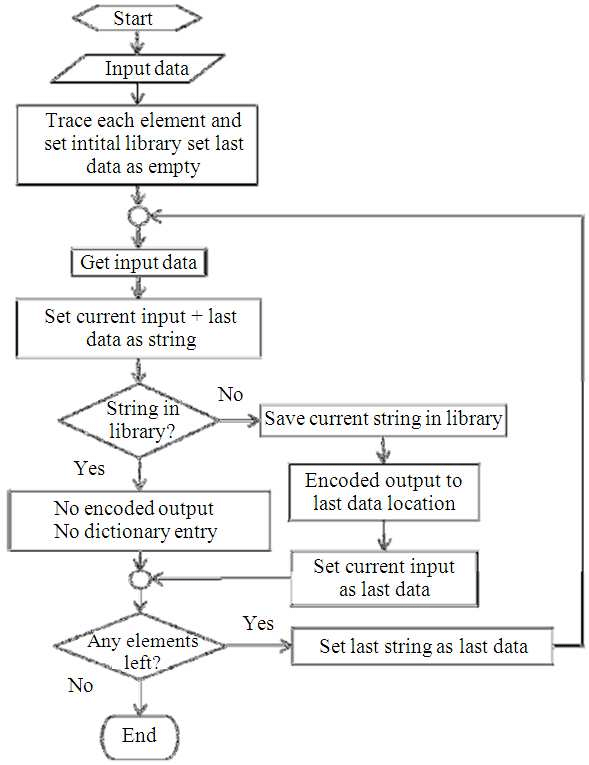
\includegraphics[width=250pt]{LZW-encoder.png}
        \vspace{1cm}
        \caption{Flowchart - Metodologia de Processamento}
        \caption{Flowchart - Codificador Utilizado}
    \end{figure}
    
\clearpage
%%%%%%%%%%%%%%%%%% Decoder Algorithm %%%%%%%%%%%%%%%%%%%%%%%%%%%%%%%%%%%%%%%%%%%%%%%&&&&&&&&&&&&&&&

\section{Descompressão}
    A descompressão dos dados é feita a partir dos dados do programa Canal e contém as seguintes funções:
    \vspace{0.5cm}
    
    \indent\textbf{1. Organize Data:}
    Esta função, tal como o nome indica, vai organizar os dados do programa Canal preparando-os para serem descodificados pelo descodificador. O seu argumento será os dados do programa.
    \vspace{0.5cm}
    
    \indent\textbf{2. Decompress:}
    Esta função recebe como argumento os dados previamente comprimidos e vai fazer a acção contrária, vai descomprimi-los de acordo com o descompressor do algoritmo de LZW.
    \vspace{0.5cm}
    
    \indent\textbf{3. Hamming Correction:}
    Esta função vai receber como argumento os dados descomprimidos pela função anterior e o resultante do ficheiro de código hamming-code.py e vai averiguar se a informação foi deturpada pelo canal. Quer isto dizer, se ouve algum bit que tenha sido trocado. Caso tenha ocorrido, então a função vai repor o bit(s) trocados na posição ou ordem correta. A aplicação e implementação do código de Hamming encontra-se feita no ficheiro de código referido.
    \vspace{0.5cm}
    
    \indent\textbf{4. Write file:}
    Esta função vai receber como argumento os dados comprimidos pela função anterior e vai escreve-la num ficheiro de extenção .txt.
    \vspace{0.5cm}
    \begin{figure}[!ht]
        \centering
        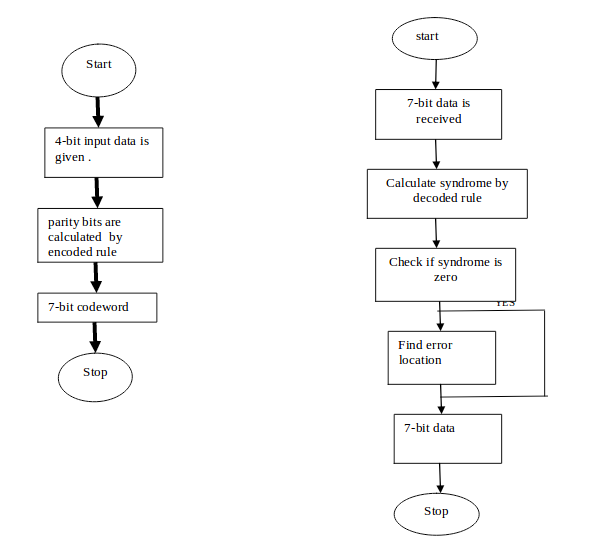
\includegraphics[width=295pt]{hamming.png}
        \caption{Flowchart - Processamento de um codigo de hamming}
    \end{figure}

    \begin{figure}[!ht]
        \flushleft
        \begin{tikzpicture}[node distance=1cm]
           \node (start) [startstop] {Inicio:Canal};
           \node (input) [io, below of=start, yshift=-0.5cm] {Input:Dados};
           \node (decoderP) [processes, below of=input, yshift=-0.5cm] {Descodificador};
           \node (decision) [decision, below of=encoderP, yshift=-2.25cm] {Dados por descomprimir?};
           \node (pp) [pp, left of=decision, xshift=-2cm]{};
           \node (hamming) [processes, below of=decision, yshift=-3cm] {Hamming};
           \node (stop) [startstop, below of=hamming, yshift=-0.55cm] {Fim: registered-values.txt};
           
           \draw [arrow] (start) -- (input);
           \draw [arrow] (input) -- (decoderP);
           \draw [arrow] (decoderP) -- (decision);
           \draw [arrow] (decision) -- node[anchor=south] {Sim} (pp);
           \draw [arrow] (pp) |- (decoderP);
           \draw [arrow] (decision) -- node[anchor=east] {Não} (hamming);
           \draw [arrow] (hamming) -- (stop);
        \end{tikzpicture}
        \centering
        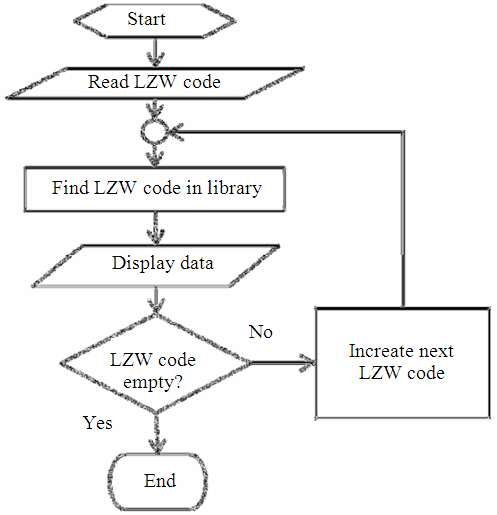
\includegraphics[width=250pt]{LZW-decoder.png}
        \vspace{1cm}
        \caption{Flowchart - Metodologia de Processamento}
        \caption{Flowchart - Descodificador Utilizado}
    \end{figure}
    
\clearpage
%%%%%%%%%%%%%%%%%% Calculus %%%%%%%%%%%%%%%%%%%%%%%%%%%%%%%%%%%%%%%%%%%%%%%%%%%&&&&&&&&&&&&&&&&&&&&

\section{Cálculos}
    \vspace{1cm}\subsection{Entropia:}
        \vspace{0.5cm}\indent Formula Utilizada: \[ H(X) = - \sum_{x E X} p(x) * \log _{2} p(x)\]
        
    \vspace{1cm}\subsection{Entropia Condicionada H(Y|X):}
        \vspace{0.5cm}\indent Formulas Utilizadas: 
        \indent \[ H(X,Y) = - \sum_{x E X, y E Y} p(x,y) * \log _{2} p(x,y)\]
        \vspace{0.5cm}\indent \[ H(Y|X) = H(X,Y) - H(X)\]

	 \vspace{0.5cm}\indent Formula Utilizada: 
        \indent\[ C = 1-Pe\] 
        \indent Onde Pe é a probabilidade de inverter um bit e C a capacidade do canal.
    
\clearpage
%%%%%%%%%%%%%%%%%% Conclusion %%%%%%%%%%%%%%%%%%%%%%%%%%%%%%%%%%%%%%%%%%%%%%&&&&&&&&&&&&&&&&&&&&&&&

\section{Balanço}
    Após a realização deste trabalho, adquirirmos um conhecimento mais consolidado acerca da matéria leccionada ao longo do semestre. Conhecimento este que passa pela implementação em código python do algoritmo seleccionado, algoritmo LZW, sob a forma de codificador e descodificador de dados provenientes da fonte e do canal, respectivamente.
    
    \vspace{1cm}\indent Como o canal é um canal com ruído, quando se obteve a informação descodificada através do algoritmo de LZW teve-se que recorrer a uma implementação adicional do código de hamming de modo a remover e restaurar, se necessário, qualquer troca de bits que possa ter ocorrido.
    
    \vspace{1cm}\indent Com os dados recolhidos pelo codificador e descodificador, será possível proceder ao calculo da entropia e entropia condicionada colocadas em prática através de uma implementação em código python. Recorrendo sempre aos conteúdos leccionadas nas aulas.
    
\clearpage
\end{titlepage}
\end{document}
